% ============================================================
%  DISCOVERY CURRICULUM — Journey 2, Module 2
%  "The Rules of Differentiation"
%  Compile with: pdflatex J2_M2.tex  (run twice for references)
% ============================================================

\documentclass[12pt, a4paper]{article}

\usepackage[a4paper, top=2.5cm, bottom=2.5cm, left=2.8cm, right=2.8cm, headheight=15pt]{geometry}
\usepackage{amsmath, amssymb, amsthm}
\usepackage{xcolor}
\usepackage{mdframed}
\usepackage{enumitem}
\usepackage{tikz}
\usetikzlibrary{arrows.meta, positioning, calc}
\usepackage{pgfplots}
\pgfplotsset{compat=1.18}
\usepackage{booktabs}
\usepackage{fancyhdr}
\usepackage{titlesec}
\usepackage{parskip}
\usepackage{hyperref}
\hypersetup{colorlinks=true, linkcolor=NavyBlue, urlcolor=NavyBlue}

% ── Colours ─────────────────────────────────────────────────
\definecolor{NavyBlue}{HTML}{1A3A5C}
\definecolor{MidBlue}{HTML}{2E6DA4}
\definecolor{Gold}{HTML}{C8922A}
\definecolor{LightBlue}{HTML}{EBF2FA}
\definecolor{LightGold}{HTML}{FDF4E3}
\definecolor{DarkGrey}{HTML}{3A3A3A}
\definecolor{BoxGreen}{HTML}{E8F5E9}
\definecolor{SidebarGrey}{HTML}{F5F5F5}

% ── Section formatting ───────────────────────────────────────
\titleformat{\section}{\Large\bfseries\color{NavyBlue}}{}{0em}{}[{\color{MidBlue}\vspace{2pt}\rule{\linewidth}{1.5pt}}]
\titleformat{\subsection}{\large\bfseries\color{MidBlue}}{}{0em}{}

% ── Header / Footer ─────────────────────────────────────────
\pagestyle{fancy}
\fancyhf{}
\fancyhead[L]{\small\color{DarkGrey}\textit{Discovery Curriculum}}
\fancyhead[R]{\small\color{DarkGrey}\textit{Journey 2 $\cdot$ Module 2}}
\fancyfoot[C]{\small\color{MidBlue}\thepage}
\renewcommand{\headrulewidth}{0.4pt}

% ── Environments ─────────────────────────────────────────────
\newmdenv[
  backgroundcolor=NavyBlue!7,
  linecolor=NavyBlue, linewidth=2pt,
  leftline=true, rightline=false, topline=false, bottomline=false,
  innerleftmargin=14pt, innerrightmargin=10pt,
  innertopmargin=10pt, innerbottommargin=10pt,
  skipabove=14pt, skipbelow=10pt
]{puzzlebox}

\newmdenv[
  backgroundcolor=LightGold,
  linecolor=Gold, linewidth=2pt,
  leftline=true, rightline=false, topline=false, bottomline=false,
  innerleftmargin=14pt, innerrightmargin=10pt,
  innertopmargin=10pt, innerbottommargin=10pt,
  skipabove=14pt, skipbelow=10pt
]{discoverybox}

\newmdenv[
  backgroundcolor=LightBlue,
  linecolor=MidBlue, linewidth=1.5pt,
  roundcorner=4pt,
  innerleftmargin=14pt, innerrightmargin=10pt,
  innertopmargin=10pt, innerbottommargin=10pt,
  skipabove=14pt, skipbelow=10pt
]{namebox}

\newmdenv[
  backgroundcolor=BoxGreen,
  linecolor=DarkGrey!35, linewidth=1pt,
  roundcorner=4pt,
  innerleftmargin=14pt, innerrightmargin=10pt,
  innertopmargin=10pt, innerbottommargin=10pt,
  skipabove=14pt, skipbelow=10pt
]{reflectionbox}

\newmdenv[
  backgroundcolor=SidebarGrey,
  linecolor=Gold, linewidth=1.2pt,
  leftline=true, rightline=false, topline=false, bottomline=false,
  innerleftmargin=12pt, innerrightmargin=10pt,
  innertopmargin=7pt, innerbottommargin=7pt,
  skipabove=10pt, skipbelow=10pt
]{thought}

\newcounter{problem}
\newenvironment{problem}[1][]{%
  \refstepcounter{problem}%
  \par\vspace{6pt}%
  \noindent\textbf{\color{MidBlue}Problem \theproblem}%
  \ifx&#1&\else\ \textit{(#1)}\fi\textbf{.}\enskip
}{\par\vspace{4pt}}

\newcounter{deepproblem}
\newenvironment{deepproblem}[1][]{%
  \refstepcounter{deepproblem}%
  \par\vspace{6pt}%
  \noindent\textbf{\color{NavyBlue}$\bigstar$\ Deep Problem \thedeepproblem}%
  \ifx&#1&\else\ \textit{(#1)}\fi\textbf{.}\enskip
}{\par\vspace{4pt}}

% ============================================================
\begin{document}
% ============================================================

\thispagestyle{empty}
\begin{center}
{\small\color{MidBlue}\textbf{DISCOVERY CURRICULUM}\quad$\cdot$\quad\textbf{JOURNEY 2: CHANGE}}

\vspace{0.6cm}
{\color{NavyBlue}\rule{\linewidth}{2pt}}
\vspace{0.5cm}

{\Huge\bfseries\color{NavyBlue}Module 2}\\[0.3cm]
{\LARGE\bfseries\color{MidBlue}The Rules of Differentiation}\\[0.4cm]
{\color{Gold}\rule{0.4\linewidth}{1.2pt}}\\[0.4cm]
{\large\itshape\color{DarkGrey}
Rules are only worth knowing when you understand\\[0.15cm]
why they cannot be otherwise.}

\vspace{1cm}
\begin{tabular}{rl}
\color{DarkGrey}\textbf{Journey}           & Journey 2 --- Change \\[4pt]
\color{DarkGrey}\textbf{Module}            & 2 of 6 \\[4pt]
\color{DarkGrey}\textbf{Prerequisites}     & J2 Module 1 (limit definition of derivative, power rule) \\[4pt]
\color{DarkGrey}\textbf{You will discover} & Sum rule, product rule, chain rule, implicit differentiation \\[4pt]
\color{DarkGrey}\textbf{Format}            & 8 problems $+$ 3 deep problems $\approx$ 13 pages \\
\end{tabular}

\vspace{1cm}
{\color{NavyBlue}\rule{\linewidth}{2pt}}
\end{center}

\vspace{0.5cm}

\noindent\textbf{The problem with first principles.}
Module~1 gave you the limit definition of the derivative and the power rule. But returning to the limit definition for every function is brutally slow. To differentiate $f(x) = x^3 \sin(x^2 + 1) \cdot e^{-x}$, you would face a limit calculation of terrifying complexity. There must be a better way.

\medskip
There is. The rules of differentiation --- sum, product, quotient, chain --- reduce differentiation of any combination of functions to a small set of algebraic moves. But these rules are not arbitrary shortcuts. Each one follows from the limit definition by a single clean argument. The goal of this module is to derive each rule, understand \emph{why} it takes the form it does, and develop fluency with it.

\newpage

% ============================================================
\section{Part 1 \texorpdfstring{---}{--} The Puzzle}
% ============================================================

\begin{puzzlebox}
\textbf{The Opening Puzzle.}

You know how to differentiate $x^2$ and $\sin x$ separately. But consider:
\[
  f(x) = x^2 \sin x.
\]

\textbf{Guess 1.} Is $(fg)' = f'g'$? Test this: differentiate $x^2 \cdot x^3 = x^5$ directly. Does $(x^2)'(x^3)' = (x^5)'$?

\textbf{Guess 2.} Is $(f \circ g)' = f' \circ g'$? That is, does differentiating the composition give the composition of the derivatives? Test with $f(x) = x^2$, $g(x) = x^3$, so $(f\circ g)(x) = x^6$.

\textbf{Both guesses are wrong.} Record the correct derivatives by working from first principles for these simple cases, and note what the actual pattern seems to be. Then read on.
\end{puzzlebox}

% ============================================================
\section{Part 2 \texorpdfstring{---}{--} Exploration}
% ============================================================

\subsection{Step 1: Sum and constant multiple}

\begin{problem}
\label{prob:sum_rule}
Let $f$ and $g$ be differentiable. Define $s(x) = f(x) + g(x)$.
\begin{enumerate}[label=(\alph*), topsep=2pt]
  \item Write out $\dfrac{s(x+h) - s(x)}{h}$ and separate it into two fractions.
  \item Take $h \to 0$ to derive: $(f + g)' = f' + g'$.
  \item Prove similarly that $(cf)' = c f'$ for any constant $c$.
  \item Use these two rules to differentiate $p(x) = 5x^4 - 3x^2 + 7x - 2$ without returning to the limit definition.
  \item The sum rule says differentiation is \emph{linear}: $\frac{d}{dx}(\alpha f + \beta g) = \alpha f' + \beta g'$. In Journey~1 you saw that integration operators on function spaces are also linear. Is differentiation an operator on a function space? What is its domain?
\end{enumerate}
\end{problem}

\subsection{Step 2: The product rule}

\begin{problem}
\label{prob:product_rule_derive}
Let $p(x) = f(x) \cdot g(x)$. We want $p'(x)$.

\begin{enumerate}[label=(\alph*), topsep=2pt]
  \item Write $p(x+h) - p(x) = f(x+h)g(x+h) - f(x)g(x)$.
  \item Add and subtract $f(x)g(x+h)$ inside this expression. Factor to get:
  \[
    p(x+h) - p(x) = g(x+h)\bigl[f(x+h) - f(x)\bigr] + f(x)\bigl[g(x+h) - g(x)\bigr].
  \]
  \item Divide by $h$ and take $h \to 0$. Use the fact that $g(x+h) \to g(x)$ (continuity from differentiability).
  \item State the product rule you have derived.
  \item \textbf{Geometric interpretation.} The product $f(x) \cdot g(x)$ is the area of a rectangle with sides $f$ and $g$. When $x$ increases by $h$, the area changes by three pieces: two thin rectangles and one tiny corner square. Draw this. Why does the corner square vanish in the limit?
\end{enumerate}
\end{problem}

\begin{center}
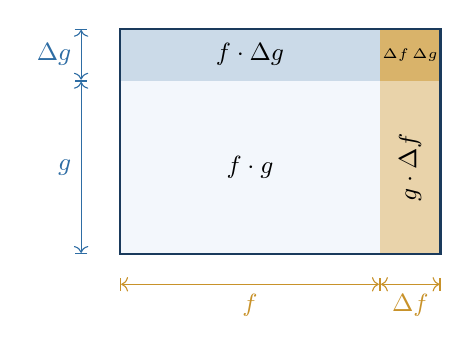
\begin{tikzpicture}[scale=1.1]
  % Main rectangle f*g
  \fill[LightBlue!60] (0,0) rectangle (3,2);
  % Right strip: delta_f * g
  \fill[Gold!40] (3,0) rectangle (3.7,2);
  % Top strip: f * delta_g
  \fill[MidBlue!25] (0,2) rectangle (3,2.6);
  % Corner: delta_f * delta_g
  \fill[Gold!70] (3,2) rectangle (3.7,2.6);
  % Labels
  \draw[thick, NavyBlue] (0,0) rectangle (3.7,2.6);
  \node at (1.5,1) {\small $f \cdot g$};
  \node at (3.35,1) {\small\rotatebox{90}{$g \cdot \Delta f$}};
  \node at (1.5,2.3) {\small $f \cdot \Delta g$};
  \node at (3.35,2.3) {\tiny $\Delta f\,\Delta g$};
  % Dimension labels
  \draw[|<->|, Gold] (0,-0.35) -- (3,-0.35) node[midway,below,font=\small] {$f$};
  \draw[|<->|, Gold] (3,-0.35) -- (3.7,-0.35) node[midway,below,font=\small] {$\Delta f$};
  \draw[|<->|, MidBlue] (-0.45,0) -- (-0.45,2) node[midway,left,font=\small] {$g$};
  \draw[|<->|, MidBlue] (-0.45,2) -- (-0.45,2.6) node[midway,left,font=\small] {$\Delta g$};
\end{tikzpicture}
\end{center}

\begin{problem}
\label{prob:product_apply}
Use the product rule to differentiate:
\begin{enumerate}[label=(\alph*), topsep=2pt]
  \item $f(x) = x^3 \cdot e^x$
  \item $g(x) = x^2 \cdot \sin x$
  \item $h(x) = (x^2 + 1)(x^3 - 2x)$ \quad [verify by expanding first]
  \item $k(x) = e^x \cdot \sin x$ \quad [the result is important --- note its form]
  \item $\ell(x) = x \cdot \ln x$ \quad [you will need $\frac{d}{dx}\ln x = 1/x$, which is derived in Problem~\ref{prob:log_deriv}]
\end{enumerate}
\end{problem}

\subsection{Step 3: The chain rule}

The chain rule is the most powerful and most frequently used rule in calculus. It tells you how to differentiate a function of a function.

\begin{problem}
\label{prob:chain_rule_derive}
Let $F(x) = f(g(x))$. We want $F'(x)$.

\begin{enumerate}[label=(\alph*), topsep=2pt]
  \item The na\"{i}ve argument: write
  \[
    F'(x) = \lim_{h\to 0}\frac{f(g(x+h)) - f(g(x))}{h}.
  \]
  Introduce $k = g(x+h) - g(x)$ and try to rewrite this as:
  \[
    \lim_{h\to 0} \frac{f(g(x)+k) - f(g(x))}{k} \cdot \frac{k}{h}.
  \]
  What do each of the two factors approach as $h \to 0$?
  \item State the chain rule: $(f \circ g)' = \,$?
  \item In Leibniz notation, if $y = f(u)$ and $u = g(x)$, the chain rule reads:
  \[
    \frac{dy}{dx} = \frac{dy}{du} \cdot \frac{du}{dx}.
  \]
  Why does this look like fractions cancelling? Is it literally a fraction? Discuss carefully.
  \item \textbf{Physical interpretation.} If temperature $T$ depends on altitude $h$, and altitude $h$ depends on time $t$ (you are ascending a mountain), then $\frac{dT}{dt} = \frac{dT}{dh} \cdot \frac{dh}{dt}$. Explain this in words. Is the chain rule obvious from this physical picture?
\end{enumerate}
\end{problem}

\begin{thought}
\textbf{The subtlety in the chain rule proof.}
The na\"{i}ve argument in Problem~\ref{prob:chain_rule_derive}(a) has a flaw: the step where we divide by $k$ fails when $k = 0$, which can happen even as $h \to 0$ (if $g$ is constant near $x$). The fix requires a more careful reformulation using the definition of differentiability, writing $f(g(x)+k) - f(g(x)) = f'(g(x)) \cdot k + \varepsilon(k) \cdot k$ where $\varepsilon(k) \to 0$ as $k \to 0$. This is the \emph{$\varepsilon$-$\delta$} approach. The na\"{i}ve argument gives the right answer and the right intuition --- but the rigorous proof requires more care. In mathematics, the intuitive argument is usually discovered first and the rigorous proof follows later, sometimes by decades.
\end{thought}

\begin{problem}
\label{prob:chain_apply}
Use the chain rule to differentiate:
\begin{enumerate}[label=(\alph*), topsep=2pt]
  \item $f(x) = (x^2 + 1)^{10}$
  \item $g(x) = e^{3x^2 - x}$
  \item $h(x) = \sin(x^3)$
  \item $k(x) = \sqrt{1 - x^2}$ \quad [relevant to the unit circle]
  \item $\ell(x) = \ln(\sin x)$
  \item $m(x) = e^{\sin(x^2)}$ \quad [chain rule applied twice]
\end{enumerate}
For each one: identify the outer function $f$ and inner function $g$ before differentiating.
\end{problem}

\subsection{Step 4: Quotient rule and derivatives of standard functions}

\begin{problem}
\label{prob:quotient}
\begin{enumerate}[label=(\alph*), topsep=2pt]
  \item Derive the quotient rule by writing $\frac{f}{g} = f \cdot g^{-1}$ and applying the product rule and chain rule (with the chain rule applied to $g^{-1}$).
  \item State the result: $\left(\frac{f}{g}\right)' = \,$?
  \item Use it to find $\frac{d}{dx}\tan x = \frac{d}{dx}\frac{\sin x}{\cos x}$. Simplify using $\sin^2 x + \cos^2 x = 1$.
  \item Differentiate $\frac{x^2 + 1}{x^3 - 1}$.
\end{enumerate}
\end{problem}

\begin{problem}
\label{prob:log_deriv}
\begin{enumerate}[label=(\alph*), topsep=2pt]
  \item We know $e^{\ln x} = x$. Differentiate both sides with respect to $x$ using the chain rule. Solve for $\frac{d}{dx}\ln x$.
  \item Use the result to differentiate $\ln(x^2 + 1)$, $\ln(\sin x)$, and $x \ln x - x$.
  \item \textbf{Logarithmic differentiation.} To differentiate $y = x^x$, take $\ln$ of both sides first: $\ln y = x \ln x$. Now differentiate both sides with respect to $x$ (using the chain rule on the left). Solve for $y'$.
  \item Use the same technique for $y = x^{\sin x}$.
  \item As $x \to 0^+$, what happens to $x^x$? Compute numerically for $x = 0.1, 0.01, 0.001$. Does the limit surprise you?
\end{enumerate}
\end{problem}

\begin{thought}
\textbf{Why the chain rule is the most important rule.}
Of the four differentiation rules, the chain rule is the one that appears most often in real applications. Almost every function encountered in physics, engineering, and statistics is a composition: $e^{-x^2/2}$ is $e^u$ composed with $u = -x^2/2$; $\sin(\omega t + \phi)$ is $\sin u$ composed with $u = \omega t + \phi$; $\ln(1+x^2)$ is $\ln u$ composed with $u = 1+x^2$. The chain rule is the rule for differentiating the world as it actually is, rather than the simple test cases. The Leibniz notation $\frac{dy}{dx} = \frac{dy}{du}\cdot\frac{du}{dx}$ is not an accident: Leibniz designed his notation specifically so that the chain rule would look like fraction cancellation, making it easier to apply correctly. This is the same Leibniz who lost the priority dispute with Newton --- and whose notation, not Newton's, is what every physicist and engineer uses today.
\end{thought}

\subsection{Step 5: Implicit differentiation}

\begin{problem}
\label{prob:implicit}
The equation $x^2 + y^2 = 1$ defines a circle. It does not define $y$ as a function of $x$ globally (it fails the vertical line test). But \emph{locally} near most points, $y$ can be treated as a differentiable function of $x$.

\begin{enumerate}[label=(\alph*), topsep=2pt]
  \item Differentiate both sides of $x^2 + y^2 = 1$ with respect to $x$, treating $y$ as a function of $x$ and applying the chain rule to $y^2$. Solve for $\frac{dy}{dx}$.
  \item Verify by solving $y = \sqrt{1-x^2}$ explicitly and differentiating. Do you get the same answer?
  \item Find $\frac{dy}{dx}$ for $x^3 + y^3 = 6xy$ (the folium of Descartes).
  \item Find the slope of the tangent to $x^3 + y^3 = 6xy$ at the point $(3, 3)$.
  \item The equation $x^2 + y^2 = 1$ represents a circle. At the point $(x_0, y_0)$ on the circle, what is the relationship between the tangent direction and the radius? Does your formula for $\frac{dy}{dx}$ confirm this?
\end{enumerate}
\end{problem}

% ============================================================
\section{Part 3 \texorpdfstring{---}{--} Discovery}
% ============================================================

\begin{discoverybox}
\textbf{What have we built?}

Four rules, each derived from the limit definition:
\[
  (f+g)' = f'+g', \quad (fg)' = f'g + fg', \quad \left(\frac{f}{g}\right)' = \frac{f'g - fg'}{g^2}, \quad (f\circ g)' = (f'\circ g)\cdot g'.
\]

Together with the base cases $\frac{d}{dx}x^n = nx^{n-1}$, $\frac{d}{dx}e^x = e^x$, $\frac{d}{dx}\sin x = \cos x$, $\frac{d}{dx}\ln x = 1/x$, these four rules let you differentiate any combination of elementary functions.

\medskip
\textbf{The deeper pattern.} The sum rule says differentiation distributes over addition. The product rule says it does not distribute over multiplication --- instead it satisfies the \emph{Leibniz rule} $(fg)' = f'g + fg'$. This is not an accident. Any operation $D$ on functions that satisfies linearity and the Leibniz rule is called a \textbf{derivation}. Derivations appear in abstract algebra, differential geometry, and the mathematics of quantum mechanics. The derivative you have been computing is one instance of a far more general algebraic concept.

\medskip
\textbf{Before reading on.} The chain rule tells you $(f\circ g)' = (f'\circ g)\cdot g'$. Differentiation is itself a kind of function: it takes a function and returns a function. It is a \emph{linear operator} on function space. Does the chain rule mean that differentiation commutes with composition? (Hint: does $(f\circ g)' = f'\circ g'$?)
\end{discoverybox}

% ============================================================
\section{Part 4 \texorpdfstring{---}{--} Naming the Ideas}
% ============================================================

\begin{namebox}
\textbf{The four differentiation rules.}

Let $f$, $g$ be differentiable functions and $c$ a constant.

\medskip
\textbf{Linearity:} $(cf + g)' = cf' + g'$

\medskip
\textbf{Product rule (Leibniz rule):} $(fg)' = f'g + fg'$

\medskip
\textbf{Quotient rule:} $\displaystyle\left(\frac{f}{g}\right)' = \frac{f'g - fg'}{g^2}$\quad (where $g \neq 0$)

\medskip
\textbf{Chain rule:} $(f \circ g)'(x) = f'(g(x))\cdot g'(x)$, \quad or in Leibniz notation: $\dfrac{dy}{dx} = \dfrac{dy}{du}\cdot\dfrac{du}{dx}$

\medskip
\textbf{Standard derivatives:}
\[
  \frac{d}{dx}x^n = nx^{n-1}, \quad
  \frac{d}{dx}e^x = e^x, \quad
  \frac{d}{dx}\sin x = \cos x, \quad
  \frac{d}{dx}\cos x = -\sin x, \quad
  \frac{d}{dx}\ln x = \frac{1}{x}.
\]
\end{namebox}

% ============================================================
\section{Part 5 \texorpdfstring{---}{--} Deep Problems}
% ============================================================

\begin{deepproblem}[Derivations in algebra]
An operation $D$ on a ring of functions is a \textbf{derivation} if it satisfies:
\begin{enumerate}[label=(\roman*), noitemsep]
  \item $D(f+g) = D(f) + D(g)$ \quad (linearity over addition)
  \item $D(fg) = D(f)\cdot g + f\cdot D(g)$ \quad (Leibniz rule)
\end{enumerate}
\begin{enumerate}[label=(\alph*)]
  \item Prove that $D(c) = 0$ for any constant function $c$, using only properties (i) and (ii).
  \item Prove that $D(f^n) = nf^{n-1}D(f)$ using (ii) and induction. This generalises the power rule.
  \item Consider the operator $D_a(f) = a \cdot f'$ for a fixed function $a$. Show this is a derivation.
  \item The commutator $[D_1, D_2] = D_1 D_2 - D_2 D_1$ of two derivations is itself a derivation. Verify this for $D_1 = \frac{d}{dx}$ and $D_2 = x\frac{d}{dx}$ by computing $[D_1, D_2](f)$ for a general $f$.
  \item In quantum mechanics, position and momentum are represented as derivations on a Hilbert space, and their commutator is proportional to the identity. This is the mathematical statement of Heisenberg's uncertainty principle. Write one sentence connecting this algebraic fact to the physical principle.
\end{enumerate}
\end{deepproblem}

\begin{deepproblem}[Inverse function theorem]
\begin{enumerate}[label=(\alph*)]
  \item If $f$ has an inverse $f^{-1}$, then $f(f^{-1}(y)) = y$. Differentiate both sides with respect to $y$ using the chain rule to derive:
  \[
    (f^{-1})'(y) = \frac{1}{f'(f^{-1}(y))}.
  \]
  \item Apply this to find the derivative of $\arcsin x$ (the inverse of $\sin$ on $[-\pi/2, \pi/2]$). Simplify using $\sin^2\theta + \cos^2\theta = 1$.
  \item Find the derivative of $\arctan x$. Sketch the graph of $\arctan x$ and verify that your answer is always positive --- what does this say about the function?
  \item The \textbf{Inverse Function Theorem} says: if $f'(x_0) \neq 0$, then $f$ is locally invertible near $x_0$ and the inverse is differentiable. Why does $f'(x_0) = 0$ prevent this? Give a geometric argument and an algebraic one.
  \item Apply the theorem to the equation $F(x, y) = x^3 + y^3 - 6xy = 0$ near the point $(3,3)$. Does an implicit function $y(x)$ exist near this point? What is $y'(3)$?
\end{enumerate}
\end{deepproblem}

\begin{deepproblem}[Taylor's theorem]
If $f$ is $n$-times differentiable, its \textbf{Taylor polynomial} at $x = a$ is:
\[
  P_n(x) = \sum_{k=0}^{n} \frac{f^{(k)}(a)}{k!}(x-a)^k.
\]
\begin{enumerate}[label=(\alph*)]
  \item Compute $P_3(x)$ for $f(x) = e^x$ at $a = 0$. How close is $P_3(0.5)$ to $e^{0.5}$?
  \item Compute $P_4(x)$ for $f(x) = \sin x$ at $a = 0$. Plot $\sin x$ and $P_4(x)$ on the same axes for $x\in[-2\pi, 2\pi]$. Where does the approximation break down?
  \item \textbf{Taylor's theorem with remainder:} $f(x) = P_n(x) + R_n(x)$ where $R_n(x) = \frac{f^{(n+1)}(c)}{(n+1)!}(x-a)^{n+1}$ for some $c$ between $a$ and $x$. Use this to bound the error in approximating $\cos(0.1)$ by $P_4(x)$ at $a=0$.
  \item Taylor polynomials are the ``best polynomial approximations'' in a precise sense. What goes wrong if you try to approximate $f(x) = |x|$ by a Taylor polynomial at $a = 0$?
  \item \textit{(Look ahead.)} The full Taylor series $\sum_{k=0}^{\infty}\frac{f^{(k)}(a)}{k!}(x-a)^k$ converges to $f(x)$ for some functions (analytic functions) but not all. Give an example of a smooth function whose Taylor series at $a=0$ converges everywhere but equals $f$ only at $a=0$.
\end{enumerate}
\end{deepproblem}

% ============================================================
\section{Part 6 \texorpdfstring{---}{--} Reflection}
% ============================================================

\begin{reflectionbox}
\textbf{Your reflection task.}

\begin{enumerate}
  \item \textbf{On the product rule.} The product rule says $(fg)' = f'g + fg'$. The rectangle diagram gives a geometric reason. Write down two more interpretations --- one algebraic, one physical (hint: think of $f$ and $g$ as quantities that change in time).

  \item \textbf{On derivations.} The deep problem showed that differentiation is one example of a derivation, an algebraic object satisfying two simple axioms. In your view, is the derivative ``really'' a limit of difference quotients, or ``really'' a derivation satisfying the Leibniz rule? Can both be true simultaneously? What does it mean for a mathematical object to be ``really'' one thing?

  \item \textbf{On Leibniz notation.} The chain rule in Leibniz notation looks like $\frac{dy}{dx} = \frac{dy}{du} \cdot \frac{du}{dx}$. This looks like the $du$ terms cancel. They do not literally cancel (they are not fractions). Yet the notation makes the rule easy to apply and almost impossible to forget. What other mathematical notations have you seen that look like they work for the wrong reasons?

  \item \textbf{Looking ahead.} Module~3 introduces the integral --- the reverse operation of differentiation. You found that $(x^2)' = 2x$. So presumably the ``anti-derivative'' of $2x$ is $x^2$. But what about $+C$? Why should the anti-derivative not be unique?
\end{enumerate}
\end{reflectionbox}

\medskip
\noindent\textbf{Looking ahead.}
Differentiation breaks a function into its rate-of-change. Module~3 goes the other direction: given the rate, reconstruct the function. This is the integral. The Fundamental Theorem of Calculus --- the central theorem of Journey~2 --- will reveal that differentiation and integration are exactly inverse operations, and that the area under a curve is computed by anti-differentiation. The connection is one of the most beautiful surprises in all of mathematics.

\vspace{1.4cm}
\begin{center}
{\color{MidBlue}\rule{0.5\linewidth}{0.8pt}}\\[6pt]
{\small\color{DarkGrey}\textit{End of Journey 2, Module 2 --- The Rules of Differentiation}}\\[4pt]
{\small\color{DarkGrey}Continue to: \textbf{Module 3 --- The Integral}}\\[6pt]
{\color{MidBlue}\rule{0.5\linewidth}{0.8pt}}
\end{center}

\end{document}